%------------------------------------------------------------------------------
% Template file for the submission of papers to IUCr journals in LaTeX2e
% using the iucr document class
% Copyright 1999-2003 International Union of Crystallography
% Version 1.2 (11 December 2002)
%------------------------------------------------------------------------------

\documentclass[preprint]{iucr}              % DO NOT DELETE THIS LINE
\usepackage{lscape}
\newcommand{\mb}[1]{\ensuremath{\mbox{\boldmath $ #1 $}}}
\newcommand{\mbss}[1]{\ensuremath{\mbox{\boldmath $ \scriptstyle #1 $}}}
\newcommand{\av}[1]{\ensuremath{\langle #1 \rangle}}
\newcommand{\dubint}{\int\!\!\!\int}
\newcommand{\intZ}{\int\!\!\!\int}

     %-------------------------------------------------------------------------
     % Information about the type of paper
     %-------------------------------------------------------------------------
     \paperprodcode{a000000}      % Replace with production code if known
     \paperref{xx9999}            % Replace xx9999 with reference code if known
     \papertype{FA}               % Indicate type of article
                                  %   FA - research papers (full article)
                                  %   SC - short communications
                                  %   FC - fast communications
                                  %   LA - lead article
                                  %   TR - topical review
                                  %   XL - crystallization papers
                                  % (Following categories rarely in LaTeX)
                                  %   AA - abstracts
                                  %   AD - addenda and errata
                                  %   AI - inorganic compounds
                                  %   AM - metal-organic compounds
                                  %   AO - organic compounds
                                  %   BC - books received
                                  %   BR - book reviews
                                  %   BI - biography
                                  %   CA - cif applications
                                  %   CD - crystal data
                                  %   CE - current events
                                  %   CI - inorganic compounds
                                  %   CL - calendar of events
                                  %   CM - metal-organic compounds
                                  %   CN - cryocrystallography papers
                                  %   CO - organic compounds
                                  %   CP - computer programs
                                  %   CR - crystallographers
                                  %   CS - scientific comment
                                  %   ED - editorial
                                  %   EI - inorganic compounds
                                  %   EM - metal-organic compounds
                                  %   EO - organic compounds
                                  %   FI - inorganic compounds
                                  %   FM - metal-organic compounds
                                  %   FO - organic compounds
                                  %   IP - issue preface
                                  %   IU - iucr
                                  %   LE - letters to the editor
                                  %   LN - laboratory notes
                                  %   ME - forthcoming meetings/short courses
                                  %   MR - meeting reports
                                  %   NN - notes and news
                                  %   NP - new commercial products
                                  %   OB - obituaries
                                  %   PA - computer program abstracts
                                  %   RI - reference information
                                  %   SG - structural genomics papers
                                  %   SI - short format inorganic compounds
                                  %   SM - short format metal-organic compounds
                                  %   SO - short format organic compounds
                                  %   SP - short structural papers
                                  %   SR - software reviews
                                  %   TE - teaching and education

     \paperlang{english}          % Can be english, french, german or russian
     %-------------------------------------------------------------------------
     % Information about journal to which submitted
     %-------------------------------------------------------------------------
     \journalcode{A}              % Indicate the journal to which submitted
                                  %   A - Acta Crystallographica Section A
                                  %   B - Acta Crystallographica Section B
                                  %   C - Acta Crystallographica Section C
                                  %   D - Acta Crystallographica Section D
                                  %   E - Acta Crystallographica Section E
                                  %   J - Journal of Applied Crystallography
                                  %   S - Journal of Synchrotron Radiation
          %--------------------------------------------------------------------
          % The following entries will be changed as required by editorial staff
          %--------------------------------------------------------------------
     \journalyr{2003}
     \journaliss{1}
     \journalvol{59}
     \journalfirstpage{000}
     \journallastpage{000}
     \journalreceived{0 XXXXXXX 0000}
     \journalaccepted{0 XXXXXXX 0000}
     \journalonline{0 XXXXXXX 0000}

\begin{document}              % DO NOT DELETE THIS LINE

\title{Molecular Crystal Global Phase Diagrams:\\ II. Reference Lattices}
%\shorttitle{Global phase diagrams II}

\cauthor[a,b]{Richard B.}{McClurg}{richard.mcclurg@aptuit.com}{}
\author[a,c,d]{J. Brandon}{Keith}%{jbrkeith@gmail.com}

\aff[a]{Department of Chemical Engineering and Materials Science, University of Minnesota, Minneapolis, Minnesota 55455, \country{USA}}
\aff[b]{SSCI, a division of Aptuit, West Lafayette, Indiana 47906 \country{USA}}
\aff[c]{Department of Physics and Astronomy, Brigham Young University, Provo, Utah 84602, \country{USA}}
\aff[d]{California Institute of Technology, Division of Engineering and Applied Science, Mail Code 138-78, Pasadena, California 91125 \country{USA}}
%\keyword{global phase diagram}

\maketitle                        % DO NOT DELETE THIS LINE

\begin{synopsis}
Experimental crystal structures that are amenable for inclusion in Global Phase Diagrams as previously developed are identified.  
\end{synopsis}

\begin{abstract}
In the first part of this series~\cite{Keith04c,Mettes04}, we developed a method for constructing global phase diagrams  (GPDs) for molecular crystals in which crystal structure is presented as a function of intermolecular potential parameters.  In that work, a FCC center of mass lattice was arbitrarily adopted as a reference state.  In part two of the series, we classify experimental crystal structures composed of tetrahedral point group molecules to determine what fraction of structures are amenable to inclusion in the GPDs and the number of reference lattices necessary to span the observed structures.  We find that 60\% of crystal structures composed of molecules with Td point group symmetry are amenable and that eight reference lattices are sufficient to span the observed structures.  Similar results are expected for other cubic point groups.
\end{abstract}


\pagebreak

\section{Introduction}

In the first part of this series, a method for constructing a global phase diagram (GPD) for molecular crystals of molecules of a given point group symmetry was developed \cite{Mettes04}.  Conventional phase diagrams present the equilibrium phase behavior of a chemical substance or of a mixture of substances as functions of thermodynamic variables such as temperature, pressure, or composition.  Global phase diagrams also present equilibrium phase behavior, but at least one of the independent variables of the diagram is either a parameter in an empirical equation of state or a parameter in an intermolecular potential.  The classic example of a GPD of the first type is the classification scheme for high pressure vapor liquid phase equilibria by van Konyenburg \cite{VanKonyenburg80}. Their classification was based on the van der Waals equation of state with simple binary mixing rules. Despite the crude equation of state employed, it is still widely used to classify the phase behavior of real binary mixtures.  Our GPDs are of the second type. They use an intermolecular potential constructed from a subset of a complete set of intermolecular potential basis functions for molecules sharing a particular point group symmetry.  The parameters of the intermolecular potential are axes on GPDs.  At the origin of each diagram is a plastic crystal phase that serves as the reference state for construction of the diagram.  In the example developed previously, \cite{Keith04c,Mettes04} a diagram was constructed for molecules of $T_d$ point group symmetry and a FCC reference lattice.  These choices were motivated in part by the classic analysis of methane phase behavior \cite{James59}.  Two independent variables were arbitrarily chosen in \cite{Keith04c} and three independent variables were chosen in \cite{Mettes04}.  

Two issues were left unresolved in the previous contribution \cite{Mettes04}.  First, the number and variety of reference lattices needed to summarize experimental crystal structures was not determined.  Although the FCC reference lattice is appropriate for cryogenic methane, it is expected that other reference lattices are required to span the diversity of observed crystal structures.  Second, the number of independent variables necessary to span the diversity of intermolecular potentials was not determined.  It has been asserted that too many parameters are needed to represent an intermolecular potential to be practical \cite{Briels80}.  This assertion was based on a particular method for associating a potential with a parameter set.  While the method employed was reasonable, it is not the only possibility.  It left open the possibility that another association would lead to a more practical parameter set dimensionality.  The first issue is addressed in this contribution while the second is addressed in a separate contribution \cite{Keith09}.

The outline of the balance of the paper is as follows. In Sec. \ref{sec:Data} we discuss the derivation of our data set, its chemical and crystallographic characteristics, and classify entries based on structural similarity. In Sec. \ref{sec:Classification} we deduce reference lattices for each structure.  The resulting assignments and their implications for use in constructing Global Phase Diagrams are discussed in Sec. \ref{sec:Discussion}.

\section{Data set}
\label{sec:Data}

Since molecular crystal global phase diagrams are constructed for molecules of a given molecular point group symmetry, we have chosen to use the \emph{CSDSymmetry} database as the primary source of crystal structures for this study~\cite{Yao02}. This database summarizes the point groups of molecules that form non-disordered, non-polymeric, non-ionic, coordinate-determined molecular crystals in the CSD.  Duplicate structures were removed from the database and hydrogen atoms were not considered when assigning point groups. While the methods introduced in our previous work~\cite{Mettes04} are applicable to disordered structures, which are systematically absent from \emph{CSDSymmetry}, it is a convenient source of crystal data for molecules of a particular point group. Our methods are restricted to single component crystals, however. Therefore we worked with the single component crystal subset of the \emph{CSDSymmetry} database.  This was accomplished by first querying the CSD for all single component crystals using {C\small ONQUEST}, the interface to the CSD, and then using {C\small ONQUEST} to take the intersection of the two data sets.

% Continuing the example begun in our prior work~\cite{Mettes04}, we chose to consider crystals composed of molecules with T$_d$ molecular point group symmetry.  We have augmented the data from \emph{CSDSymmetry} with a recently determined structure of the low temperature ordered phase of heavy methane~\cite{Neumann03}.  The data set contains 71 crystal structures of 70 different chemical substances.  Only carbon tetrachloride ($\mathrm{CCl}_4$) appeared twice in different polymorphs. [CSD structures CARBTC~\cite{Piermarini73} and CARBTC07~\cite{Cohen79}]. The chemical structures include 15 hydrocarbons and their substituted derivatives and 56 organometallics. The organometallics contain 30 different metals: Al, As, Bi, Cd, Co, Cs, Cu, Ga, Ge, Hf, In, Mg, Mn, Na, Ni, Np, Pb, Pt, Re, Rh, Ru, Sb, Si, Se, Sn, Tc, Th, Ti, U, and Zn.  Eight molecular framework types are present in the data set: Cubane (29), Adamantane (17), MX$_4$ (16), Tetrahedrane (3), and others (6).  There are entries from all seven crystal systems in the data set. Twenty crystals are cubic (also called isometric), one is hexagonal, five are trigonal, ten are tetragonal, six are orthorhombic, twenty-two are monoclinic, and seven are triclinic (also called anorthic) as illustrated in Fig.~\ref{fig_provenance}.  
% 
% Eight molecular framework types are present in the data set: Cubane (29), Adamantane (17), MX$_4$ (16), Tetrahedrane (3), and others (6).
% 
% This distribution is different than the CSD as a whole~\cite{Baur92}, but that is not surprising given the larger-than-average number of symmetries in the T$_d$ point group.  The data set is sufficient however to test whether molecular crystal global phase diagrams apply to organic and organometallic molecules, a variety of molecular frameworks, and all seven crystal systems.

Continuing the example begun in our prior work~\cite{Mettes04}, we chose to consider crystals composed of molecules with T$_d$ molecular point group symmetry.  We have augmented the data from
\emph{CSDSymmetry} with a recently determined structure of the low temperature ordered phase of heavy methane~\cite{Neumann03}.  The data set contains 71 crystal structures of 70 different chemical substances.  Only carbon tetrachloride ($\mathrm{CCl}_4$) appeared twice in different polymorphs. [CSD structures CARBTC~\cite{Piermarini73} and CARBTC07~\cite{Cohen79}]. Names and chemical formulas for all the entries are given in (supplementary) Table 9 available from the publisher. The chemical structures include 15 hydrocarbons and their substituted derivatives and 56 organometallics. The organometallics contain 30 different metals: Al, As, Bi, Cd, Co, Cs, Cu, Ga, Ge, Hf, In, Mg, Mn, Na, Ni, Np, Pb, Pt, Re, Rh, Ru, Sb, Si, Se, Sn, Tc, Th, Ti, U, and Zn. Eight molecular framework types, also shown in (supplementary) Table 9, are present in the data set: Cubane (29), Adamantane (17), MX$_4$ (16), Tetrahedrane (3), and others (6). There are entries from all seven crystal systems in the data set. Twenty crystals are cubic (also called isometric), one is hexagonal, five are trigonal, ten are tetragonal, six are orthorhombic, twenty-two are monoclinic, and seven are triclinic (also called anorthic) as illustrated in Figure~\ref{distro}. This distribution is different than the CSD as a whole~\cite{Baur92}, but that is not surprising given the larger-than-average number of symmetries in the T$_d$ point group.  The data set is sufficient however to test whether molecular crystal global phase diagrams apply to organic and organometallic molecules, a variety of molecular frameworks, and all seven crystal systems.


\subsection{Space Group Assignment Corrections}
\label{corrections}

Several researchers have shown that structures with incorrect space group assignments account for at least 3\% of the entries in the Cambridge Structural Database (CSD).\cite{Baur86,Marsh95}  Given the size of the test set used in this study, it is to be expected that a few errors must be identified and corrected.

CSD entry JUFWUC \cite{Tesh92} appears to have been incorrectly assigned to space group $P23$ (no. 195) rather than $P\bar{4}3m$ (no. 215).  Both space groups are members of the generic cubic extinction symbol P\,-\,-\,-.  Thus they have no systematic extinctions and thus x-ray diffraction peaks occur in all of the same positions for both groups.  They belong to different Laue classes however.  Space group 195 is in Laue class $m\bar{3}$ while space group 217 is in $m\bar{3}m$.  Space group 195 is a subgroup of 215 of order two.  The symmetry operation present in 215, but missing in 195 is a face-diagonal mirror plane.  The fractional coordinates for the Cs, N, and Si atoms provided by the authors are all consistent with the existence of the ``missing" mirror plane.  The fractional coordinates of the carbon atoms are very nearly consistent with the existence of the mirror plane and are within the indicated error given by the authors.  The hydrogen atom positions provided in JUFWUC.cif were calculated and not determined experimentally.  Therefore they do not provide independent evidence of the crystal symmetry.  Evidently the structure was determined under space group 195, but space group 215 cannot be ruled out based on the authors’ own estimates of the uncertainties in the fractional coordinates.  It is standard practice to accept the higher symmetry space group in this case.

CSD entry HMGETP \cite{Dahl75} appears to have been incorrectly assigned to space group $I23$ (no. 197) rather than $I\bar{4}3m$ (no. 217).  Both space groups are members of the generic body-centered cubic extinction symbol I\,-\,-\,-.  Thus they have the same systematic extinctions and thus x-ray diffraction peaks occur in all of the same positions for both groups.  They belong to different Laue groups however.  Space group 197 is in Laue class $m\bar{3}$ while space group 217 is in $m\bar{3}m$.    Space group 197 is a subgroup of 217 of order two.  The symmetry operation present in 217, but missing in 197 is a face-diagonal mirror plane.  The fractional coordinates for the Ge and P atoms provided by the authors are all consistent with the existence of the ``missing" mirror plane.  The fractional coordinates of the carbon atoms are very nearly consistent with the existence of the mirror plane.  Since no error estimate for the fractional coordinates was provided by the authors, the distance from the given atomic position to the proposed mirror plane was calculated as an indication of the difference between the reported symmetry and the proposed symmetry.  Adjusting the carbon atom positions by 0.0049\AA{} along two coordinate directions restores the ``missing" mirror plane.  This is well within the resolution of the structure determination.  No hydrogen atom positions were provided in HMGETP.cif.  Evidently the structure was determined under space group 197, but space group 217 cannot be ruled out based on a reasonable estimate of the uncertainties in the fractional coordinates.  It is standard practice to accept the higher symmetry space group in this case.

It is interesting to note that both of the above structures appear to have been mistakenly assigned to a lower-than-necessary space group due to the omission of a face-diagonal mirror plane.  Assignment of the structure to the incorrect space group is due to the incorrect Laue point group assignment.  This is a type 2 error in the nomenclature of Baur and Tillmanns \cite{Baur86}.  In such cases, the reported structure is very similar to the presumed correct structure.  Correcting the error requires only adjusting the reported atomic fractional coordinates and changing the reported space group.

One entry [CSD structure XUWROW~\cite{Sung02}] is a very unusual structure containing 70\% voids as recorded by the CCDC staff in the corresponding cif file in the CSD.  Although low density sphere packings are possible, stability requires that each sphere be surrounded by at least four neighbors that are not in the same hemisphere \cite{Conway98}.  Structure XUWROW has large voids separating layers of molecules parallel to the \{001\} plane.  Molecules at the edges of the layers have all of their neighbors in a single hemisphere and therefore violate a necessary condition for sphere packing stability.  Also, the layers are separated by wide voids in the reported structure.  Dispersion interactions between the layers would tend to narrow these wide void layers.  For these reasons, it seems likely that the reported crystal structure is mechanically unstable.  According to the original publication, the crystal was grown as a thin epitaxial crystal under ultra-high vacuum.  Apparently the crystal structure is either strongly influenced by the substrate which stabilizes the crystal or the structure was not determined correctly.  In either case, it is not an independent stable form we therefore exclude it from further consideration.


\section{Classification}
\label{sec:Classification}

Neglecting CSD structure XUWROW and reassigning structures JUFWUC and HMGETP as discussed above, the remaining crystal structures were organized into groups that bear a strong ``structural relation" as discussed in the first edition of Volume C of the International Tables for Crystallography (ITC) \cite{Hahn83}. For crystals to belong to the same group they must have the same space group symmetry, cell lengths in similar proportions, similar cell angles, and molecular centers at equivalent Wyckoff point(s) with similar structural parameter values where applicable.  Crystal structures with alternative origin and/or cell choices were transformed to consistent cell and origin choices prior to assessing their structural relationship, if any.  For monoclinic space groups, cell choice 1 with unique axis $b$ was utilized.  For Rhombohedral space groups, the obverse setting of the hexagonal cell was utilized.  Origin choice 2 was utilized in cases where more than one origin is provided in the International Tables for Crystallography.  For molecules located at Wyckoff points that belong to an equivalent set, preference was given to the label occurring first alphabetically.  Thus, Wyckoff point $a$ was selected rather than $b$ in space group $P\bar{4}2_1c$ (no. 114) since both are equivalent.  We refer to the members of these structurally related groups as sharing a distinct structure. Note that we do not require that the atomic positions be similar to be classified in the same distinct structure. For example, two structures [CSD structures DILWIE01~\cite{Ebert98} and ZEYHIU~\cite{Noth95}] crystallize in space group $P\bar{3}c1$ (no. 165) with molecular centers at Wyckoff point $d$. Their cell parameters are also in similar ratios. Therefore, we classify them in the same distinct structure, despite their different chemical structures with different numbers of atoms.

The 70 crystal structures fall into 46 distinct structures. Five structures are cubic (\textit{aka} isometric), one is hexagonal, four are trigonal, eight are tetragonal, six are orthorhombic, sixteen are monoclinic, and six are triclinic (\textit{aka} anorthic).  These distinct structures are further characterized based on the number and relative positions of neighboring centers-of-mass in the following subsections.  The center-of-mass lattice is used here to be consistent with the reference state employed in the prior work \cite{Keith04c,Mettes04}.  In the fully orientationally disordered reference state only the center-of-mass distances are relevant.  As the temperature is reduced, the systems undergo symmetry-breaking phase transitions through orientation of the constituent molecules.  For the oriented molecules the closest contacts and/or the strongest interactions may be with molecules that are not nearest neighbors with respect to centers-of-mass.  The interactions are addressed in \cite{Keith04c,Mettes04} while this work focuses solely on the assignment of the reference lattice.

\subsection{Sphere Packings}

In 42 structures there are four or more neighbors that are equidistant or nearly equidistant.  Also, the neighbors are not all in one hemisphere relative to the (arbitrary) reference molecule.  Such structures are identified as sphere packings \cite{Conway98}, and classified by the space group symmetry of the center-of-mass lattice.  The center-of-mass lattice is called the reference lattice for brevity and for consistency with our prior work \cite{Keith04c,Mettes04}.  The structures and their reference lattices are tabulated in Table \ref{tab_sphere}.

For 15 crystal structures, assignment of the reference lattice is trivial since the unit cell shares the same Bravais symmetry as the reference lattice and the molecules sit at high symmetry locations in the crystal.  This is true of the structures in space groups $Fd3m$ (no. 227), $I\bar{4}3m$ (no. 217), and $P\bar{4}3m$ (no. 215) with Diamond Cubic, Body-Centered Cubic, and Simple Cubic reference lattices, respectively.  

The body-centered cubic space group $I\bar{4}3m$ (no. 217) with molecules at Wyckoff point $a$ is the most common structure in the data set with 11 different crystal structures.  The CSD structure labeled NIWMIP is used as an example of that structure in Figure \ref{fig_NIWMIP}.  The vertical axis in the figure is the symmetry density defined as the ratio of the order of the symmetry group to the number of molecules.  Along the horizontal axis are insets showing the molecular structure on the left, the reference lattice on the right, and the crystal structure in the middle.  The diagram shows symmetry breaking during creation of the crystal.  For a symmetry breaking, the ratio of the symmetry density prior to and after the transitions gives the index of the transition.  To facilitate visual comparisons of transition indices, the symmetry density is plotted on a logarithmic scale in the figures.  Figure \ref{fig_NIWMIP} conveys that the full molecular symmetry is retained while the BCC reference lattice symmetry is broken in forming the structure in space group 217.  The broken symmetry is the inversion which yields an index of two.

The four crystal structures assigned to the HCP reference lattice are all slightly compressed along the c-axis relative to the expectation for ideal close-packing of spheres.  This is consistent with the observation for many other HCP structures \cite{Sands93}.  Of the elements that adopt HCP structures, only helium adopts the ideal unit cell dimension ratio, $c/a=(8/3)^{1/2}$.  Cadmium and zinc adopt elongated unit cells with $c/a>(8/3)^{1/2}$.  Twenty two other elemental solids adopt slightly compressed HCP structures with $c/a<(8/3)^{1/2}$.  Despite variation in the unit cell dimension ratios, these elements are commonly described as adopting the HCP crystal structure.  We utilize the same flexibility in nomenclature when assigning the HCP reference lattices to molecular solids.

For 23 crystal structures, symmetry breaking in passing from the reference lattice to the observed structure leads to dramatic changes in the conventional unit cell size and/or shape.  Reference lattice assignment in these cases is not trivial.  The CSD structure labeled MEZDIE01 serves to illustrate the process.  MEZDIE01 has a triclinic unit cell in space group $P\bar{1}$ (no. 2) with molecular centers at the general Wyckoff point $i$.  The alpha and gamma angles of the unit cell are very close to 90 degrees, so that the unit cell is metrically similar to a monoclinic cell, but the connection to a BCC reference lattice is not immediately evident.  The fractional coordinates of the molecular centers-of-mass are very close to one-quarter and three-quarters of the distance along a cell body diagonal.  If the molecular centers were at precisely these locations, and molecular orientational ordering is ignored, then the unit cell of the reference lattice can be halved in volume using a matrix transformation.  The resulting unit cell has one molecular center per reduced cell.  The reduced cell is nearly equi-axed (cell lengths differ from the mean by less than 1\%) and nearly rhombohedral (angles differ from the mean by less than 1 degree).  The reduced cell belongs to character number 44 (triclinic), but is only slightly distorted from character 5 (BCC).  Applying the standard matrix transformation (for character 5) from the reduced cell to the conventional cell yields the reference lattice.  The product of the two matrix transformations gives the overall transformation from the reference lattice to the observed crystal structure.  Finally, the overall transformation matrix is confirmed using COPL \cite{Stokes07}.  COPL confirms that all of the symmetry elements present in the daughter structure are inherited from the reference lattice, confirms the index of the transformation, and provides the complete order parameter list for the transformation.  The matrix unit cell representations and matrix transformations used in determining the reference lattice assignment starting with MEZDIE01 are given in an Appendix.  The same information for each of the structures identified with sphere packing reference lattices and their associated COPL outputs are summarized in (supplementary) Table 8.

Six crystal structures were identified with the diamond reference lattice.  Only one of these, ZNOXAC01, retains the cubic unit cell with four nearest neighbors for each molecular center.  The other five are significantly distorted.  Two are compressed, one is elongated, and two are orthorhombically distorted similar to the $\gamma$-Plutonium structure with ten equidistant neighbors \cite{NRL08}.  These distortions may be due to the low packing density of the ideal diamond cubic lattice relative to the other reference lattices.

\subsection{Rod Packings}

In 16 crystal structures there are two neighbors that are equidistant or nearly
equidistant and the third neighbor is significantly further away than the second.  In an additional six crystal structures, there are three or four equidistant or nearly equidistant neighbors, but these neighbors are all in a single hemisphere.  For all 16 crystal structures, a synthon based on one-dimensional chains of molecules have been identified.  Here the term synthon is used to refer to substructures present in crystal structures.  A similar concept is described by Lauher \cite{Lauher04} and called networks.  Chains of molecules are classified by their rod symmetries \cite{Hahn02VolE}.  Classification of the structures in these cases requires identification of the rod symmetry and the lateral packing motif.

The CSD structure labeled MECKIO is used as an example of a crystal structure composed of rods.  Its symmetry breaking plot is illustrated in Figure \ref{fig_MECKIO}.  The inset on the left is an isolated monomer with $Td$ symmetry (G/Z=24/1).  Second from the left is a rod packing with rod group $p\bar{4}m2$ (G/Z=8/1).  The inset on the far right is a two-dimensional hexagonal packing representing the lateral packing of the rods (G/Z=12/1).  Second from the right is the crystal structure with one rod emphasized for clarity (G/Z=4/2).  The crystal is viewed end-on to emphasize nearly hexagonal packing of rods.  The symmetry density decreases at each stage of building the crystal from its constituents.  

All of the crystal structures composed of laterally packed rods are summarized in Table \ref{tab_rods}.  In the subset of crystal structures containing rod packings, five different rod symmetries were identified, $pmcm$ (7/16, 44\%), $p\bar{4}m2$ (4/16, 25\%), $p\bar{1}$ (4/16, 25\%), and $pc11$ (1/16, 6\%).  The majority of the rods packed laterally in hexagonal close-packing (9/16, 56\%) while a significant fraction adopted a square packing (6/16, 38\%), and only one example of a decidedly oblique packing (1/16, 6\%) was observed.  A total of eight combinations of rod symmetries and lateral packings were observed.

In the CSD structure labeled RIMNAC the rods have $p\bar{4}m2$ symmetry and adopt a nearly hexagonal lateral packing, but there are three independent rotations about the rod axis.  These three rotations lead to three independent Wyckoff orbits.  This is in contrast to most of the other structures in the data set for which the orientations of the rods are related by symmetry operations of the three-dimensional crystal.

\subsection{Planar Packings}

In five structures there are three or four neighbors that are equidistant or nearly equidistant and the next neighbor is significantly further away than the second.  Also, the neighbors are either coplanar or in one hemisphere relative to the (arbitrary) reference molecule.  Such structures are identified as planar packings, and classified by their planar group symmetry \cite{Hahn02VolE}.  The structures and their planar group symmetries are tabulated in Table \ref{tab_planes}.  

The CSD structure labeled MZNMOX10 is used as an example of a crystal structure composed of planes of molecules.  Its symmetry breaking plot is illustrated in Figure \ref{fig_MZNMOX10}.  The inset on the left is an isolated monomer with $Td$ symmetry (G/Z=24/1).  On the far right is a two-dimensional square packing representing the center-of-mass lattice in the plane (G/Z=8/1).  Second from the right is a planar packing with point group $S4$ (G/Z=4/1).  Because the molecules are tipped slightly in the three-dimensional crystal, the plane is not viewed along its normal in the inset, but is viewed along the molecular S4 axis to emphasize the symmetry of the undistorted planar packing.  Second from the left is the crystal structure with one plane emphasized for clarity (G/Z=4/4=1).  The vertical axis indicates that symmetries are broken at each stage.

\subsection{Dimer Packings}

In three structures there is one closest neighbor and the next closest neighbor is significantly further away than the first.  Such structures are identified as dimer packings, and classified by their dimer point group symmetry.  The structures and their dimer point group symmetries are tabulated in Table \ref{tab_dimers}.  

FOJBUB02 and VADRAU are cubic structures in space group $Pa\bar{3}$ (no. 205) with molecules at Wyckoff point $c$, which has $C3$ point group symmetry.  Their second nearest neighbors are 33\% and 25\% further than the closest, respectively.  Therefore, we consider these dimers as the synthon for the crystal.  The dimer centers of mass are at Wyckoff point $a$, with $C3i$ point group symmetry.  The dimer centers of mass form a perfect face centered cubic lattice.  The symmetry breaking plot for FOJBUB02 is given in Figure \ref{fig_FOJBUB02}.  The symmetries of the monomer and the FCC reference lattice are broken in creating the crystal, but the dimer symmetry is retained in the three-dimensional crystal.

LUFYEQ is a tetragonal structure in space group $I4_1/a$ (no. 88) with molecules at the general Wyckoff point, $f$.  Since the second nearest neighbor is 33\% further than the first, there are dimers serving as synthons for the crystal.  The dimers reside at Wyckoff point $e$, with $C2$ point group symmetry.  Each dimer has one neighboring dimer that is closer than any other.  Therefore, the dimers pair to produce quadramers at Wyckoff point $a$, with $S4$ point group symmetry.  The quadramer center of mass lattice is a somewhat compressed diamond cubic structure.

CARBTC is a fourth structure identified as a dimer packing, but this assignment is less apparent from the histogram of neighbor distances.  In the structure, each molecule has one nearest neighbor and two additional neighbors that are 6\% further.  This is insufficient for a sphere packing and the arrangement of molecules is inconsistent with simple planar packings.  Therefore, the packing was analyzed using dimers centered at an inversion of space group $P2_1/c$ (no. 14).

\subsection{Mixed}

Three crystal structures belonging to a common distinct structure do not fit in the above classification system because molecules residing at different Wyckoff positions have different numbers of nearest neighbors.  Structures KOXKOX, SENLAY, and RUQMEV are cubic structures in space group $P\bar{4}3n$ (no. 218) with molecules at Wyckoff positions $a$ and $c$.  The structures are tabulated in Table \ref{tab_mixed}.  The molecules at Wyckoff position $c$ form rods with rod group $p\bar{4}m2$ running parallel to all three orthogonal coordinate directions.  The molecules at Wyckoff position $a$ each have twelve equidistant nearest neighbors in a slightly distorted icosahedral coordination.  Although there are other crystal structures with multiple Wyckoff orbits in the data set, these three structures differ because the coordination of nearest neighbors is qualitatively different for the two sets.  In the other examples, the neighbor histograms are only subtly different when comparing the various orbits.  



\section{Discussion and Conclusions}
\label{sec:Discussion}

Identification of lower-dimensionality synthons as a means of describing three-dimensional crystals has been discussed previously \cite{Lauher04}.  The crystal structures identified here as rod packings have been called $\alpha$-networks and planar packings have been called $\beta$-networks in the nomenclature of \cite{Lauher04}.  The molecules used by Lauher to illustrate sub-periodic networks were polar and their intermolecular interactions had strong hydrogen bonding and/or ionic character.  Formation of strongly bound one-dimensional structures is common, but not universal, in such cases.  Two types of two-dimensional structures were identified by Lauher.  The first is a two-dimensional synthon composed of parallel one-dimensional rods, called $\alpha$-networks.   The second is a fundamentally two-dimensional structure without $\alpha$-network substructures.  In all of his examples, three dimensional crystal structures were composed of one- or two-dimensional networks.

Given the cubic point group symmetry (Td) of the molecules considered here, we expected that the corresponding crystal structures would be composed of molecules having multiple equidistant and isoenergetic interactions with four or more neighbors leading to sphere packings or $\gamma$-networks in Lauher's nomenclature.  This expectation proved accurate for 60\% (42/70) of the structures.  Of these, BCC (16/42, 38\%) and FCC (12/42, 29\%) were the most common reference lattices.  HCP and SC reference lattices contributed 10\% (4/42) each.  Only one structure (2\%) adopted the ideal diamond cubic lattice, but five structures (12\%) were identified with three grossly distorted diamond cubic structures.  Together, these eight reference lattices span the observed diversity of crystal structures based on sphere packings and are illustrated in Figure \ref{fig_provenance} under the ``Sphere Packing'' trunk.

Somewhat unexpected was the 40\% (32/70) of structures that adopted lower-dimensionality synthons.  The next largest subset of the crystal structures were composed of rods.  They comprised 23\% (16/70) of the structures.  A total of eight combinations of rod symmetries and lateral packings were observed.

Smaller fractions of other structures were assigned.  Five cases (5/70, 7\%) of planar structures, also called $\beta$-networks were observed.  Four cases (3/70, 4\%) of spherical packings of dimers and one case (1/70, 1\%) of a spherical packing of quadramers were assigned.  Finally, three isostructural examples (3/70, 4\%) of a mixed sphere and rod packing in space group $P\bar{4}3n$ (no. 218) belonged to the data set.  Given the small numbers of these structural types, their relative proportions may not be accurately determined in this set of data.  Also, the possibility of unobserved structural motifs cannot be excluded.  Figure \ref{fig_provenance} shows lower-dimensional and oligomer sythons under the ``Other'' trunk, which are further broken down to specialized types of rod packings and so on.

The goals of the research described in this report was to determine the frequency of sphere packings which are readily amenable to inclusion in the global phase diagrams (GPDs) developed previously \cite{Keith04c,Mettes04}.  In the set of crystal structures composed of molecules in the $Td$ point group, 60\% are amenable to inclusion in the global phase diagrams using the molecule as the synthon.  Eight reference lattices span the diversity of observed center of mass lattices so that a set of at least eight global phase diagrams are required to represent the phase behavior of the sphere packing subset of the data set.  Dimer and quadramer packing structures are also suitable for inclusion in GPDs using the point group symmetry of the synthon.  These account for another 6\% of the crystal structures.  Similar proportions are expected for molecular symmetries belonging to other cubic point groups.  

A qualitatively different set of phase diagrams are required for the structures that adopt lower-dimensionality synthons (rod and planar packings) or mixed structures.  The presence of such structures implies a hierarchy of interaction strengths.  We expect that strong interactions lead to the rods while weaker interactions are responsible for lateral packing of the rods into crystals.  Such a hierarchy of interaction strengths is expected for molecules belonging to lower molecular point group symmetries.  Therefore for non-cubic point group symmetries, it is expected that the proportion of crystal structures classified as sphere packings would be smaller and the proportion of rod and planar packings would be greater than that reported here for tetrahedral molecules.  


\ack{This work received financial support from the American Chemical Society - Petroleum Research Fund (PRF \#41774-AC10), DOE Grant No. DE-FG02-03ER46059, and NSF Grant DMR-0520547.
%
Computational resources maintained by the University of Minnesota Supercomputer Institute were used for portions of this research.}

\appendix
\section{Sphere Packings }

For 42 of the 70 crystal structures in the data set considered, the center of mass distribution was identified with a sphere packing.  For 15 of these, the identification was trivial since the unit cell has the same symmetry as the idealized sphere packing.  For the remaining 27 structures, the center of mass distribution is slightly distorted from the idealized sphere packing.  The process of identifying the sphere packing is not trivial in these cases because unit cell distortions and/or translation of the centers of mass change the symmetry of the center of mass lattice.  To illustrate the process of reference lattice assignment, the CSD structure MEZDIE01 is considered in detail below.  Details of the reference lattice assignments for all 42 structures are summarized in (supplementary) Table 6 and accompanying notes available from the journal publisher.

CSD structure MEZDIE01 has a triclinic unit cell with $b/a=1.4627$, $c/a=0.9209$, $\alpha=90.48\deg$, $\beta=111.67\deg$, and $\gamma=89.99\deg$.  The unit parameters can be conveniently represented in matrix form where the matrix columns correspond to the cell vectors and the rows are components of the vectors parallel to orthonormal laboratory frame coordinates,
\begin{equation}
   \mathbf{M}_1=\left[
     \begin{array}{ccc}
        1& 0.0003& -0.3401\\
        0& 1.4627& -0.0076\\
        0& 0& 0.8558\\
     \end{array}
  \right].
\end{equation}

The molecular centers of mass are located at fractional coordinates, $x=0.7606$, $y=0.2506$, and $z=0.2418$ and at the location related by inversion about the cell body center.  Unit cell transformations are facilitated using four dimensional vectors in which the fourth component is unity.
\begin{eqnarray}
   \mbox{\boldmath$\nu$}_1&=&\left[
     \begin{array}{c}
        0.7606\\
        0.2506\\
        0.2418\\
        1\\
     \end{array}
  \right]\\
   \mbox{\boldmath$\nu$}^\prime_1&=&\left[
     \begin{array}{c}
        1\\
        1\\
        1\\
        2\\
     \end{array}
  \right]-\mbox{\boldmath$\nu$}_1.
\end{eqnarray}

Enumeration of the neighboring centers of mass for an arbitrarily chosen reference molecule reveals that there are six neighbors within a shell 3\% larger than the nearest neighbor distance and two additional neighbors within a shell 11\% larger than the nearest neighbor distance.  These neighboring molecular centers are neither coplanar nor are they all in a single hemisphere.  Therefore, the molecular centers satisfy the conditions for a (slightly distorted) sphere packing reference lattice.

Recognizing that the molecular center fractional coordinates are nearly one-quarter and three-quarters of the distance along a body diagonal suggests that a matrix transformation with determinant equal to one-half is needed to generate the reduced cell for the reference lattice with one molecule per cell.  The following matrix transformation suffices for the current example,
\begin{eqnarray}
   \mathbf{T}_{12}&=&\left[
     \begin{array}{ccc}
        1/2& 1/2& 0\\
        1/2& -1/2& 0\\
        1/2& 1/2& -1\\
     \end{array}
  \right]\\
   \vert\mathbf{T}_{12}\vert&=&1/2.
\end{eqnarray}
Such transformations may be generated by inspection of the neighbor coordinates relative to the chosen reference center or by using the LePage software as implemented in the CheckCell program, for example \cite{CheckCell04}.

The matrix representation of the reduced cell is given by the matrix product of the original matrix representation and the transformation matrix,
\begin{equation}
\mathbf{M}_{1}\cdot\mathbf{T}_{12}=\left[
     \begin{array}{ccc}
        0.3301& 0.3298& 0.3401\\
        0.7276& -0.7352& 0.0076\\
        0.4279& 0.4279& -0.8558\\
     \end{array}
  \right]
\end{equation}
The reduced cell has $b/a=1.0066$, $c/a=1.0161$, $\alpha=108.00\deg$, $\beta=107.31\deg$, and $\gamma=107.084\deg$.  Construction of the Niggli matrix indicates that this triclinic cell (character 44) is reasonably close to the reduced cell corresponding to the body-centered cubic cell (character 5) \cite{Hahn02VolASec9.2}.  For the idealized character 5 reduced cell, $b/a=c/a=1$ and $\alpha=\beta=\gamma=cos^{-1}(-1/3)\approx 109.47\deg$.  For the experimental reduced cell, the angles are roughly two degrees smaller than the ideal value which indicates that the primary distortion is rhombohedral.  Smaller perturbations lead to slightly unequal unit cell length and angle parameters.

To determine the fractional coordinates of the centers of mass in the transformed coordinates, it is convenient to define an augmented transformation matrix as follows,
\begin{equation}
   \mathbf{S}_{12}=\left[
     \begin{array}{cc}
        \mathbf{T}_{12}& \mathbf{w}_{12}\\
        \mathbf{0}& \mathbf{1}\\
     \end{array}
  \right]
\end{equation}
where $w_{12}$ is the origin shift in the original coordinate system.  In this case,
\begin{equation}
   \mathbf{w}_{12}=\left[
     \begin{array}{c}
        3/4\\
        1/4\\
        1/4\\
     \end{array}
  \right].
\end{equation}
Then the transformed coordinates are given by 
\begin{eqnarray}
   \mbox{\boldmath$\nu$}_{2}&=&\mathbf{S}_{12}^{-1}\cdot
\mbox{\boldmath$\nu$}_{1}=\left[
     \begin{array}{c}
        0.0112\\
        0.0100\\
        0.0188\\
	1\\
     \end{array}
  \right]\\
   \mbox{\boldmath$\nu$}_{2}^\prime&=&\mathbf{S}_{12}^{-1}\cdot
\mbox{\boldmath$\nu$}_{1}^\prime=\left[
     \begin{array}{c}
        -0.0112\\
        -1.0100\\
       -1.0188\\
	1\\
     \end{array}
  \right]
\end{eqnarray}
both of which are reasonably close to the origin, modulo integer translations of the unit cell.

Since the reduced cell is close to the character 5 conditions with one molecule close to the origin, the sphere packing is identified with the BCC reference lattice.  Applying the tabulated transformation of the reduced cell to the conventional cell, \cite{Hahn02VolASec9.2}
\begin{eqnarray}
   \mathbf{T}_{23}&=&\left[
     \begin{array}{cccc}
        0.5 & -1 & -0.5 & 0\\
        0.5 &  1 & -0.5 & -0.5\\
        0.5 &  0 &  0.5 & -0.5\\
	  0   &  0 &  0   & 1\\
     \end{array}
  \right]\\
   \vert\mathbf{T}_{23}\vert&=&2
\end{eqnarray}
yields the matrix representation of the conventional unit cell,
\begin{equation}
   \mathbf{M}_{3}=\mathbf{M}_{2}\cdot\mathbf{T}_{23}=\left[
     \begin{array}{ccc}
        0.6699& 0.6702& 0.6599\\
        -0.7276& 0.7352& -0.0076\\
        -0.4279& -0.4279& 0.8558\\
     \end{array}
  \right].
\end{equation}
As anticipated above, the cell is slightly distorted from an ideal cubic cell, primarily by a rhobohedral distortion ($b/a=1.005$, $c/a=1.003$, $\alpha=86.5\deg$, $\beta=86.0\deg$, $\gamma=85.2\deg$).

Since the center of mass is at the origin in both the reduced cell and the BCC reference lattice, there is no need for another origin shift and the augmented transformation matrix is
\begin{equation}
   \mathbf{S}_{23}=\left[
     \begin{array}{cc}
        \mathbf{T}_{23}& \mathbf{0}\\
        \mathbf{0}& \mathbf{1}\\
     \end{array}
  \right].
\end{equation}
The overall transformation from the reported crystal structure of MEZDIE01 to the BCC reference lattice is the matrix product of the stepwise transformations,
\begin{eqnarray}
   \mathbf{S}&=&\mathbf{S}_{12}\cdot\mathbf{S}_{23}=\left[
     \begin{array}{ccc}
        0& 1& 1\\
        1& 0& 1\\
        1& 1& 0\\
     \end{array}
  \right]\\
   \vert\mathbf{S}\vert&=&1
\end{eqnarray}
and the transformed coordinates are given by
\begin{eqnarray}
   \mbox{\boldmath$\nu$}_{3}&=&\mathbf{S}^{-1}\cdot
\mbox{\boldmath$\nu$}_{1}
=\left[
     \begin{array}{c}
        0.0088\\
        0.0100\\
        0.0012\\
	1\\
     \end{array}
  \right]\\
   \mbox{\boldmath$\nu$}_{3}^{\prime\prime}&=&\mathbf{S}^{-1}\cdot
\left(\mbox{\boldmath$\nu$}_{1}+\left[\begin{array}{c}1\\
0\\
0\\
0\end{array}\right]\right)=\left[
     \begin{array}{c}
        0.5088\\
        0.5100\\
        0.5012\\
	1\\
     \end{array}
  \right].
\end{eqnarray}
The determinant of the overall transformation $|\mathbf{S}|$ is unity so that the volumes of the initial cell and the reference lattice cell are the same in this case.  Both contain two molecules, but they are paired differently as reflected in the use of primes in the center of mass coordinates, 
$\mbox{\boldmath$\nu$}_{1}^{\prime}$, 
$\mbox{\boldmath$\nu$}_{2}^{\prime}$, and
$\mbox{\boldmath$\nu$}_{3}^{\prime\prime}$.
Both molecular centers of mass are within 1\% of the unit cell dimensions of their idealized locations at the origin and cell body center, respectively.  In the idealized BCC lattice, each lattice point has eight equidistant nearest neighbors.  The rhombohedral distortion accounts for the two neighbors that are somewhat more distant than the closest six.  Other minor distortions lead to small differences in the distances to the closest six neighbors.

COPL can be used to verify that the overall transition is consistent with the
symmetries of the reference lattice and the daughter structure \cite{Stokes07}.
In addition, COPL provides a complete list of order parameters for the transition.  If a single order parameter with the appropriate size and index appears on the list, then it is identified as the primary order parameter.  Otherwise, it is identified as a coupled transformation.  For the example of MEZDIE01, there is no single primary order parameter consistent with the size (2) and index (48) of the transformation, so the transformation is coupled.  The program ISODISPLACE may be used to identify the primary order parameter for coupled transitions \cite{ISODISPLACE06}.  Since this identification was not necessary for our purposes, no attempt to further characterize the required coupling was attempted for coupled transformations.  COPL output for each of the structures identified with sphere packing reference lattices are summarized in (supplementary) Table 8 available from the journal publisher.


\section{Rod Packing }

For 16 of the 70 crystal structures in the data set considered, the center of mass distribution was identified with a rod packing.  To illustrate the process of reference lattice assignment, the CSD structure MECKIO is considered in detail below.  Details of the assignments for all 16 structures are summarized in (supplementary) Table 6 available from the journal publisher.

CSD structure MECKIO has a monoclinic unit cell with $b/a=1.6109$, $c/a=1.1271$, and $\beta=104.95\deg$.  The unit parameters can be conveniently represented in matrix form where the matrix columns correspond to the cell vectors and the rows are components of the vectors parallel to orthonormal laboratory frame coordinates,
\begin{equation}
   \mathbf{M}_1=\left[
     \begin{array}{ccc}
        1& 0& -0.2908\\
        0& 1.6109& 0\\
        0& 0& 1.0889\\
     \end{array}
  \right].
\end{equation}

The molecular centers of mass are related by a screw axis,
\begin{eqnarray}
   \mbox{\boldmath$\nu$}_{1}&=&\left[
     \begin{array}{c}
        0.2050\\
        1/4\\
        0.2193\\
	1\\
     \end{array}
  \right]\\
   \mbox{\boldmath$\nu$}_{1}^{\prime}&=&\left[
     \begin{array}{c}
        1\\
        1\\
        1\\
	2\\
     \end{array}
  \right]-\mbox{\boldmath$\nu$}_{1}.
\end{eqnarray}
Enumeration of the neighboring centers of mass for an arbitrarily chosen reference molecule reveals that there are two equidistant nearest neighbors.  Two additional neighbors are within a shell 3\% larger than the nearest neighbor distance, but the set of four neighbors are all within a single hemisphere relative to the reference center.  Therefore, the set of four neighbors do not indicate a sphere packing.

The nearest neighbors are part of a chain of molecules oriented along the crystallographic a-axis.  Therefore, the unit cell is transformed such that the chains are directed along the c-axis, and the other axes are orthogonal.  A matrix accomplishing the desired transformation is
\begin{eqnarray}
   \mathbf{T}_{12}&=&\left[
     \begin{array}{ccc}
        0& 0.2908& 1\\
        1& 0& 0\\
        0& 1& 0\\
     \end{array}
  \right]\\
   \vert\mathbf{T}_{12}\vert&=&1.
\end{eqnarray}
A subsequent rotation about the chain axis orients the chain symmetry elements relative to the a- and b-axes and rescales those axes,
\begin{eqnarray}
   \mathbf{T}_{23}&=&\left[
     \begin{array}{ccc}
        0.5814& 0.5814& 0\\
        -0.8600& 0.8600& 0\\
        0& 0& 1\\
     \end{array}
  \right]\\
   \vert\mathbf{T}_{23}\vert&=&1.
\end{eqnarray}
The product of the transformation matrices gives the overall transformation matrix,
\begin{equation}
\mathbf{T}=\mathbf{T}_{12}\cdot\mathbf{T}_{23}.
\end{equation}

To determine the fractional coordinates of the centers of mass in the transformed coordinates, it is convenient to define an augmented transformation matrix as follows:
\begin{equation}
   \mathbf{S}=\left[
     \begin{array}{cc}
        \mathbf{T}& \mathbf{w}\\
        \mathbf{0}& \mathbf{1}\\
     \end{array}
  \right]
\end{equation}
where $w$ is the origin shift in the original coordinate system,
\begin{equation}
   \mathbf{w}=\left[
     \begin{array}{c}
        0.2050\\
        1/4\\
        0.2193\\
     \end{array}
  \right].
\end{equation}
Transforming the atomic coordinates using $S$ shows that the molecular centers of mass are at Wycoff point $a$ and molecular mirror planes coincide with Wycoff point $f$ of rod group $p\bar{4}2m$.  Considering only the x and y coordinates of the rods yields a close approximation to a hexagonal ($p6mm$ planar group) projection.  Therefore, MECKIO is characterized as a hexagonal packing of $p\bar{4}2m$ rods.


\section{Other Packings}

Twelve of the 70 crystal structures in the data set considered were identified as planar packings, dimer packings, or mixed packings.  The procedures for characterizing these structures are similar to those illustrated above for sphere and rod packings.  Therefore, details are not given here, but may be found in (supplementary) Table 6 available from the journal publisher.

\referencelist[thesisbibAltered]

     %-------------------------------------------------------------------------
     % TABLES
     %-------------------------------------------------------------------------

\begin{table}
\label{tab_sphere}
\caption{Sphere Packings}
\begin{tabular}{ccccl} % Alignment for each cell: l=left, c=center, r=right
Parent & S.G. & W.P. & $|G|/Z$& CSD Code(s) \\
\hline
Diamond 	& Fd3m (no. 227) & a 	& 24 	& ZNOXAC01 \\
Diam. - Compr. & I41/amd (no. 141) & a & 8	& FUZLUH, VAFWAA \\
Diam. - Elong.	& I41/a	(no. 88)	 & a 	& 4	& KANGUB01 \\
Diam - Ortho.	& C2/c (no. 15) & e	& 2	& RASDOE, TFMETH02 \\
BCC		& I-43m (no. 217) & a 	& 24 	& DEQPAQ, HMGETP, HMSIPA \\
&		&	& 	& HXMTAM07, KELREY, MESIAD \\
&		&	& 	& MPTHOT01, NIWMIP, POSLOY10 \\
&		&	& 	& TMEPTC, YEYQAU \\
& R3c (no. 161) & a	& 3	& TCYMET \\
& Pbcn (no. 60) & c,d	& 2/3	& YIMWEW \\
& P-1 (no. 2) & i	& 1	& MEZDIE01, MEZDOK01 \\
& P-1 (no. 2) & i,i,i	& 1/3	& OHABEE \\
SC		& P-43m (no. 215) & a 	& 24 	& FOHCUA, FUZVOL, JUFWUC \\
		& I-4c2 (no. 120) & c	& 4	& YEMRIR \\
HCP		& P63/m (no. 176) & h	& 2	& CUCZUV \\
		& P-3c1 (no. 165) & d	& 3	& DILWIE01, ZEYHIU \\
		& P-3 (no. 147) & d	& 3	& ZIZHIZ \\
FCC		& P3121 (no. 152) & b	& 2	& MTRETC10 \\
		& I-42m (no. 121) & a	& 8	& ZZZKDW01 \\
		& I41/acd (no. 142) & a & 4	& KUJSIR \\
		& P-421c (no. 114) & a	& 4	& ADAMAN08, GERHOA \\
		& Cmce (no. 64) & d,f	& 1	& (MethaneIII) \\
		& C2/c (no. 15) & e	& 2	& REKYUB \\
		& C2/m (no. 12) & i	& 2	& MECKOU \\
		& P21/c (no. 14) & e	& 1	& MECKUA \\
		& P21/c (no. 14) & e	& 1	& TOHSUE \\
		& C2/c (no. 15)	& f,f,f,f	& 1/4	& CTBROM, CARBTC07 \\
\hline
\end{tabular}
\end{table}

\begin{table}
\caption{Rod Packings}
\label{tab_rods}
\begin{tabular}{cccccl}     % Alignment for each cell: l=left, c=center, r=right
S.G. 	& Molecule 	& Rod 		& Latteral & $|G|/Z$& CSD Code(s) \\
	& Wyck. Pt. 	& Symmetry 	& Packing \\
\hline
P42/nmc (no. 137) & a & p-4m2 & 8	& square & FUZTEZ \\
Pnma (no. 62) & c & pmcm	& 2	& square & GUTCED, JEYSEL,RIMMOP \\
C2/c (no. 15) & e & p-4m2	& 2	& hexagonal & BOGMEP \\
C2/c (no. 15)	& e & pmcm	& 2	& hexagonal & MSISUL10, TMGEHS10, TMSNHS10 \\
P21/m (no. 11) & e & p-4m2	& 2	& hexagonal & MECKIO \\
P21/c (no. 14) & e & pc11	& 2	& hexagonal & QUGBOJ \\
P21/c (no. 14) & e & p-1	& 1	& hexagonal & DOCNIS \\
P21/c (no. 14) & e & p-1	& 1	& square & TMSIAD \\
P21/c (no. 14) & e,e & pmcm	& 1/2	& hexagonal & MXSNOX \\
P2/c (no. 13) & e,f,g & p-4m2	& 1/2 	& hexagonal & RIMNAC \\
P-1 (no. 2) & i 	& p-1		& 1	& square & BASXOI \\
P-1 (no. 2) & i 	& p-1		& 1	& oblique & XAGXAE \\
\hline
\end{tabular}
\end{table}

\begin{table}
\caption{Planar Packings}
\label{tab_planes}
\begin{tabular}{ccccl}      % Alignment for each cell: l=left, c=center, r=right
S.G. & Molecule & Planar & $|G|/Z$& CSD Code(s) \\
	& Wyck. Pt. & Symmetry \\
\hline
P212121 (no. 19) & a &  p4mm	& 1	& MZNMOX10 \\
P21/c (no. 14) & e & p2gg	& 1	& CAMPOV, VAVYAS \\
P21/c (no. 14) & e,e & p6mm	& 1/2	& CANFIG, MXSNOX \\
P-1 (no. 2) & i,i,i,i & p6mm	& 1/4	& CANFOM \\
\hline
\end{tabular}
\end{table}

\begin{table}
\caption{Dimer Packings}
\label{tab_dimers}
\begin{tabular}{ccccl}      % Alignment for each cell: l=left, c=center, r=right
S.G. & Molecule & Dimer & $|G|/Z$& CSD Code(s) \\
& Wyck. Pt. & Wyck. Pt. \\
\hline
Pa-3 (no. 205) & c (3) & a (-3)	& 3	& FOJBUB02, VADRAU \\
I41/a (no. 88) & f (1) & e (2)*	& 1	& LUFYEQ \\
P21/c (no. 14) & e (1) & a (-1)	& 1	& CARBTC \\
\hline
\end{tabular}
\\ 
* Pairs of dimers form quadramers with $S4$ point group symmetry centered at Wyckoff point $a$.
\end{table}

\begin{table}
\caption{Mixed Packings}
\label{tab_mixed}
\begin{tabular}{cccl}      % Alignment for each cell: l=left, c=center, r=right
S.G. & W.P. & $|G|/Z$& CSD Code(s) \\
\hline
P-43n (no. 218) & a,c & 3	& KOXKOX, SENLAY, RUQMEV \\
\hline
\end{tabular}
\end{table}



     %-------------------------------------------------------------------------
     % FIGURES
     %-------------------------------------------------------------------------

\begin{figure}
\begin{center}
%\scalebox{.5}{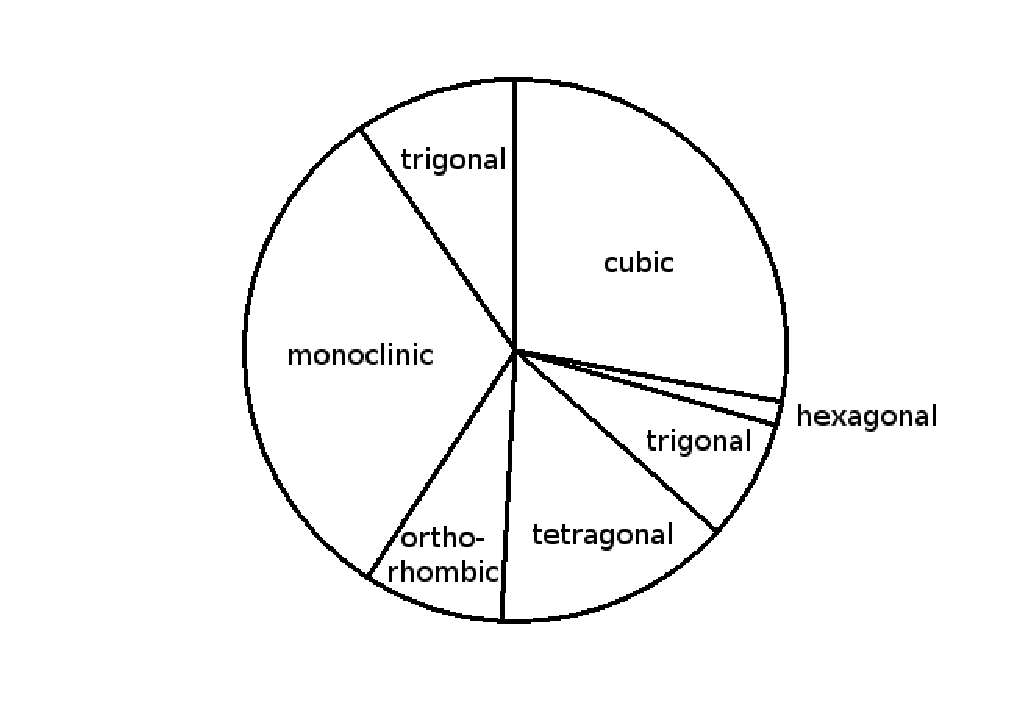
\includegraphics{crystalSystems.eps}}
\caption{Crystal systems for crystals of tetrahedral
molecules.}
\end{center}
\label{distro}
\end{figure}

\begin{figure}
\caption{Symmetry breaking plot for a structure with molecular center of mass lattice coincident with the reference lattice, illustrated using NIWMIP.  The figure on the left is an isolated monomer with $Td$ symmetry (G/Z=24/1).  The figure on the right is the BCC reference lattice (G/Z=96/2).  In the middle is the crystal structure in space group $I\bar{4}3m$ (no. 217) with one molecule at Wyckoff point $a$ emphasized for clarity (G/Z=48/2).}
\label{fig_NIWMIP}
%\scalebox{1.8}{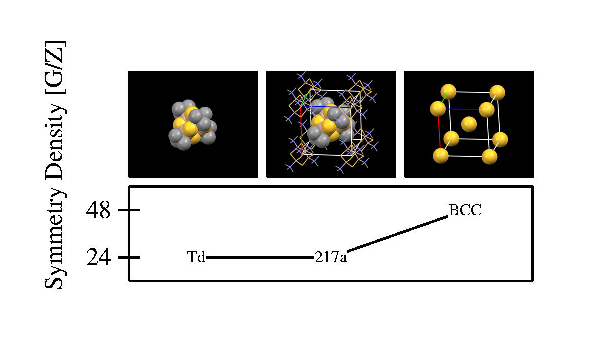
\includegraphics{217a_NIWMIP_illust.eps}}
\end{figure}

\begin{figure}
\caption{Symmetry breaking plot for a molecular center of mass lattice not trivially related to the reference lattice, illustrated using MEZDIE01.  The figure on the left is an isolated monomer with $Td$ symmetry (G/Z=24/1).  The figure on the far right is the BCC reference lattice (G/Z=96/2).  Second from the right is the BCC reference lattice in a non-conventional unit cell which may be obtained through a series of perturbations.  The illustrated cascade of symmetry-breaking transitions from BCC through tetragonal (139a), orthorhombic (69a), monoclinic (12a), and triclinic (2a) intermediates is not unique.  The non-conventional unit cell is similar to the crystal structure with one molecule emphasized for clarity in the second illustration from the left (G/Z=2/2).}
\label{fig_MEZDIE01}
%\scalebox{1.8}{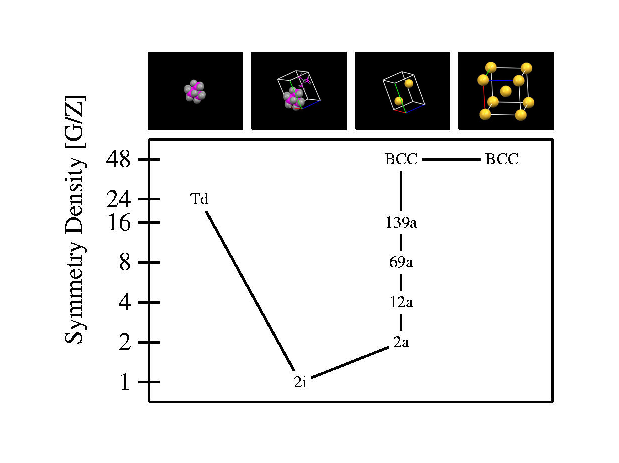
\includegraphics{2i_MEZDIE01_illust.eps}}
\end{figure}

\begin{figure}
\caption{Symmetry breaking plot for a rod packing, illustrated using MECKIO.  The figure on the left is an isolated monomer with $Td$ symmetry (G/Z=24/1).  Second from the left is a rod packing with rod group $p\bar{4}m2$ (G/Z=8/1=8).  The figure on the far right is a two-dimensional hexagonal packing representing the lateral packing of the rods (G/Z=12/1).  Second from the right is the crystal structure with one rod emphasized for clarity (G/Z=4/2).  The crystal is viewed end-on to emphasize nearly hexagonal packing of rods.}
\label{fig_MECKIO}
%\scalebox{1.8}{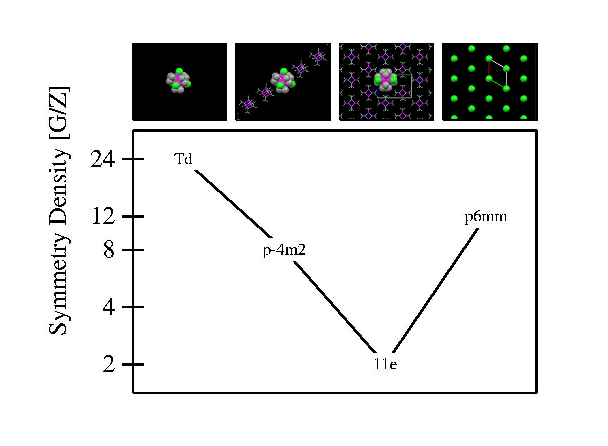
\includegraphics{11e_MECKIO_illust.eps}}
\end{figure}

\begin{figure}
\caption{Symmetry breaking plot for a planar packing, illustrated using MZNMOX10.  The figure on the left is an isolated monomer with $Td$ symmetry (G/Z=24/1).  On the far right is a two-dimensional square packing representing the center-of-mass lattice in the plane (G/Z=8/1).  Second from the right is a planar packing with point group $S4$ (G/Z=4/1).  Second from the left is the crystal structure with one plane emphasized for clarity (G/Z=4/4).}
\label{fig_MZNMOX10}
%\scalebox{1.8}{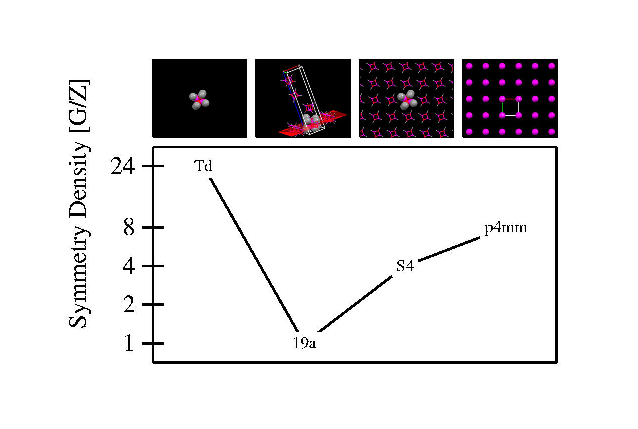
\includegraphics{19a_MZNMOX10_illust.eps}}
\end{figure}

\begin{figure}
\caption{Symmetry breaking plot for a dimer packing, illustrated using FOJBUB02.  The figure on the left is an isolated monomer with $Td$ symmetry (G/Z=24/1).  Second from the left is a dimer with $C3i$ point group symmetry (G/Z=6/2).  On the far right is the FCC reference lattice (G/Z=192/4).  Second from the right is the crystal structure in space group 205 with one dimer at Wyckoff point $a$ emphasized for clarity (G/Z=24/8).}
\label{fig_FOJBUB02}
%\scalebox{1.8}{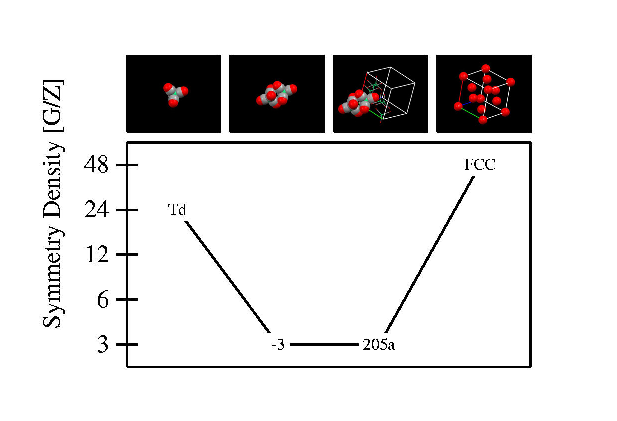
\includegraphics{205c_FOJBUB02_illust.eps}}
\end{figure}

\begin{figure}
\caption{Tree diagram of the distribution of data set among crystal packing synthons, where spheres and other types of packing form the trunk and the translational arrangements of the structures in our data set form the leaves. \scriptsize{Note: Asterisks on JUFWUC and HMGETP are due to space group corrections.  See Sec. \ref{corrections} for details.}}
\label{fig_provenance}
%\scalebox{.7}{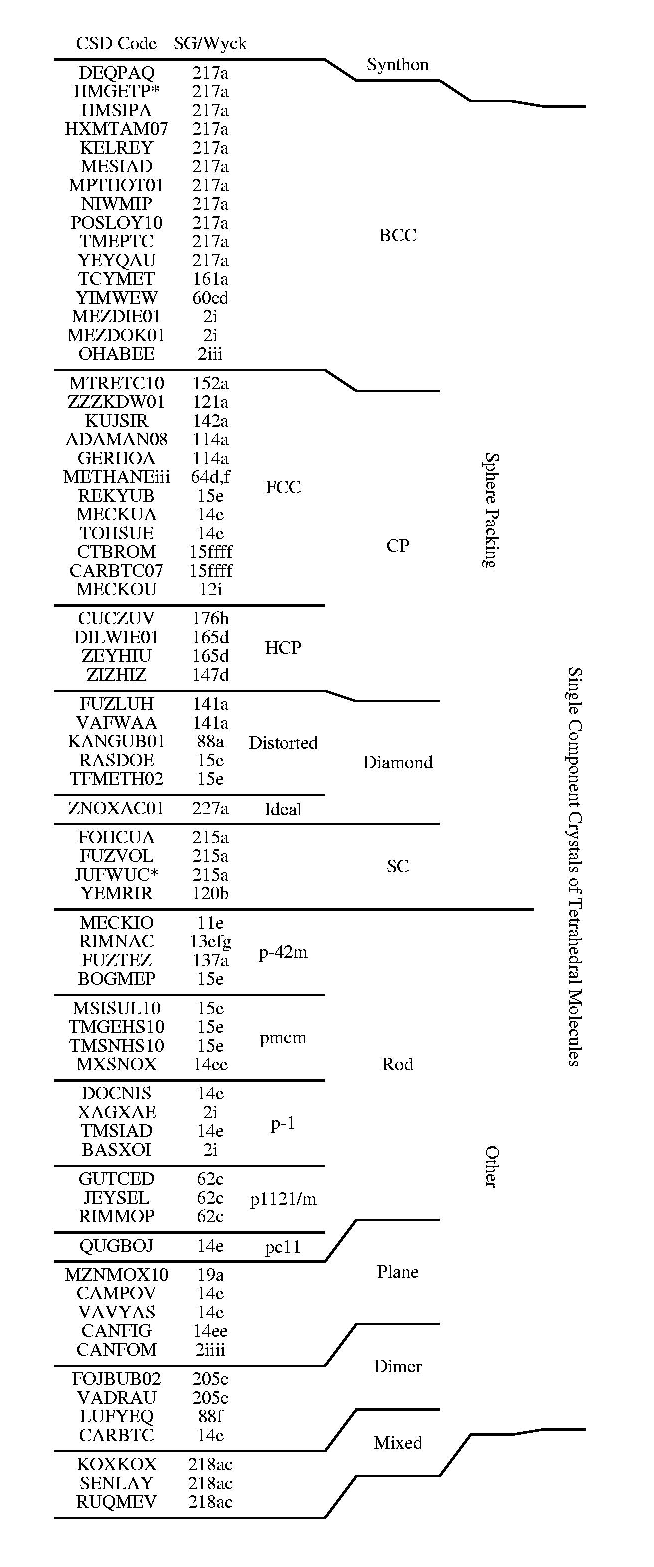
\includegraphics{breakdown_illust.eps}}
\end{figure}


\end{document}                    % DO NOT DELETE THIS LINE
%%%%%%%%%%%%%%%%%%%%%%%%%%%%%%%%%%%%%%%%%%%%%%%%%%%%%%%%%%%%%%%%%%%%%%%%%%%%%%
